\section{Results}\label{sec:results}
Each descriptor was profiled on each problem with $R = 6$ transformed replicates and $B = 60$ refit-bootstrap draws (seed 42). The primary analysis uses the within-fold AUC with class-balanced participant folds; the same profiles with the pooled AUC are a sensitivity analysis. Table~\ref{tab:auc} gives the observed AUCs with their permutation $p$-values, and Tables S1--S13 in Online Resource 1 give every profile with its intervals. Figure~\ref{fig:profiles} shows three of the profiles.

\begin{figure}[!htbp]
\centering
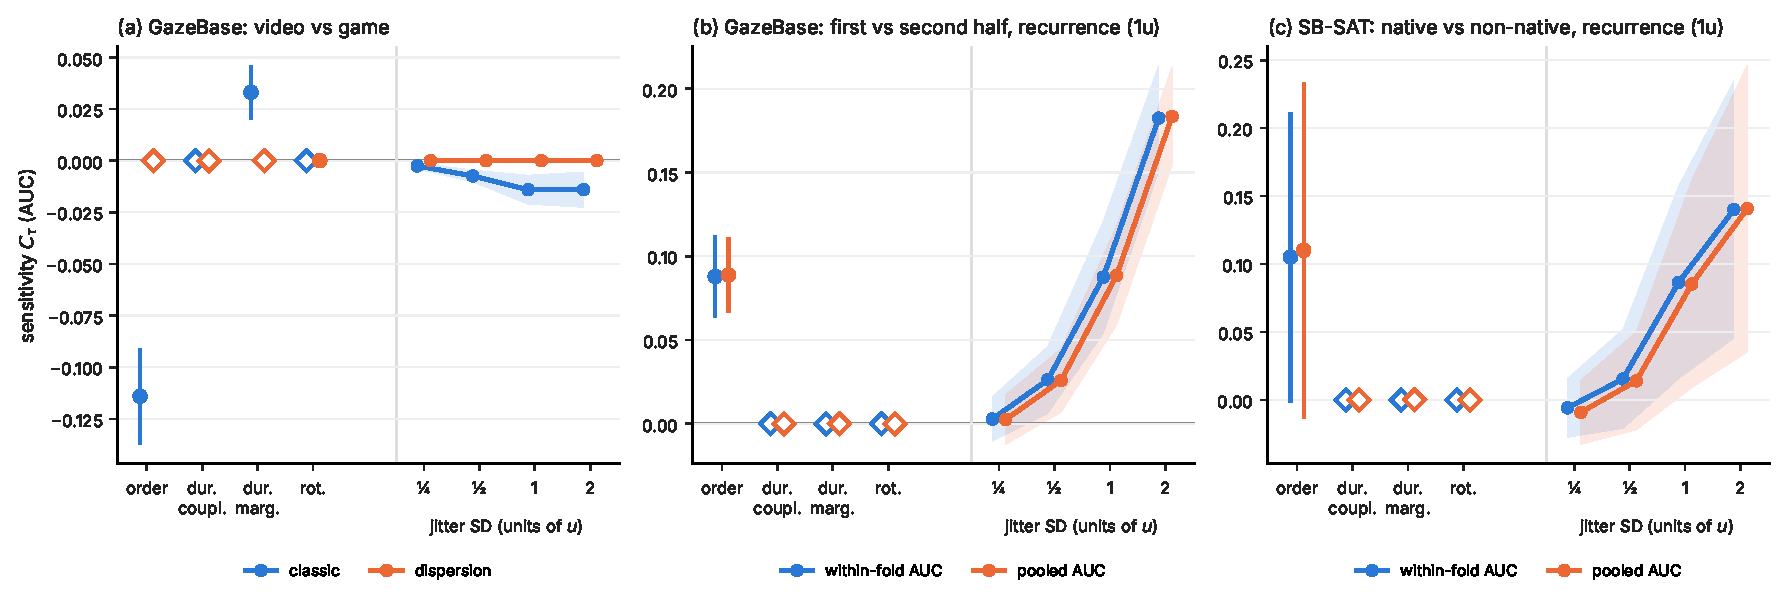
\includegraphics[width=\linewidth]{fig_profiles}
\caption{Three perturbation profiles from the real data (within-fold AUC, class-balanced folds; $R = 6$, $B = 60$). Points: sensitivity $\Cs_\tau$ with its 95\% refit-bootstrap interval for the four transformations other than jitter; open diamonds: exact invariances (the transformed features equal the observed ones, so $\Cs_\tau = 0$ with no interval); curves and bands: the jitter sweep, with jitter SD in units of the reference scale $u$. (a) GazeBase video versus game: the classic descriptor gains discrimination when order is permuted, while the dispersion baseline is order-invariant by construction. (b) GazeBase first versus second half of a video: recurrence at $1u$ under the within-fold and the pooled AUC; the two profiles nearly coincide. (c) SB-SAT native versus non-native readers, recurrence at $1u$: the jitter sensitivity at $1u$ and $2u$ excludes zero under both metrics, whereas the order sensitivity does not.}
\label{fig:profiles}
\end{figure}

\subsection{Invariance Checks}
Every analytically required invariance held exactly: every transformation for count; order for dispersion and for the undirected graph descriptors; both duration transformations for every descriptor that does not read durations, and duration coupling for the classic descriptor, which reads only their mean; rotation for recurrence and for the classic descriptor. In each case the transformed feature matrix equalled the observed one in every replicate.

\begin{table}[!htbp]
\centering\small
\caption{Observed participant-held-out AUC per problem and descriptor (within-fold AUC; class-balanced folds; linear SVM; ten-fold cross-validation over participants), with the permutation $p$-value in brackets (1000 permutations under the schemes of Table~\ref{tab:perm}; smallest attainable value 0.001). On \texttt{em\_correct} and \texttt{sb\_compr} the permutation scheme preserves part of the stimulus structure, so the permutation mean can lie well above 0.5 (Table S15) and an AUC must be read against its $p$-value. Pooled AUCs are in Table S14. A dash: descriptor not applicable.}
\label{tab:auc}
\resizebox{\linewidth}{!}{\begin{tabular}{lrrrrrrrrrr}
\toprule
Problem & Count & Dispersion & Classic & Dur.\ trend & RQA $0.5u$ & RQA $1u$ & Directed & FAG lattice & FAG AOI & FAG AOI pad. \\
\midrule
\texttt{gb\_tex\_vd1} & 0.969 (.001) & 1.000 (.001) & 0.969 (.001) & 0.957 (.001) & 0.999 (.001) & 1.000 (.001) & 0.977 (.001) & 0.988 (.001) & -- & -- \\
\texttt{gb\_vd1\_blg} & 0.690 (.001) & 1.000 (.001) & 0.886 (.001) & 0.752 (.001) & 0.999 (.001) & 1.000 (.001) & 1.000 (.001) & 0.957 (.001) & -- & -- \\
\texttt{gb\_vd1\_vd2} & 0.634 (.001) & 0.707 (.001) & 0.640 (.001) & 0.790 (.001) & 0.677 (.001) & 0.719 (.001) & 0.700 (.001) & 0.664 (.001) & -- & -- \\
\texttt{gb\_vd1\_halves} & 0.500 (1.000) & 0.924 (.001) & 0.564 (.001) & 0.590 (.001) & 0.743 (.001) & 0.823 (.001) & 0.805 (.001) & 0.741 (.001) & -- & -- \\
\texttt{gb\_tex\_s1s2} & 0.530 (.013) & 0.519 (.243) & 0.539 (.003) & 0.549 (.010) & 0.576 (.001) & 0.521 (.134) & 0.531 (.090) & 0.591 (.001) & -- & -- \\
\texttt{sb\_native} & 0.624 (.003) & 0.545 (.169) & 0.689 (.001) & 0.654 (.005) & 0.614 (.005) & 0.669 (.002) & 0.614 (.008) & 0.587 (.023) & -- & -- \\
\texttt{sb\_compr} & 0.554 (.763) & 0.413 (.975) & 0.587 (.990) & 0.575 (.929) & 0.497 (.914) & 0.529 (.919) & 0.533 (.897) & 0.506 (.810) & -- & -- \\
\texttt{em\_program} & 0.561 (.014) & 0.957 (.001) & 0.539 (.104) & 0.540 (.227) & 0.580 (.025) & 0.547 (.140) & 0.655 (.001) & 0.658 (.001) & 0.778 (.001) & 0.729 (.001) \\
\texttt{em\_halves} & 0.500 (1.000) & 0.616 (.001) & 0.776 (.001) & 0.582 (.009) & 0.613 (.001) & 0.680 (.001) & 0.634 (.001) & 0.599 (.001) & 0.682 (.001) & 0.669 (.001) \\
\texttt{em\_expertise} & 0.472 (.591) & 0.469 (.683) & 0.438 (.748) & 0.541 (.409) & 0.419 (.794) & 0.416 (.803) & 0.366 (.886) & 0.447 (.756) & 0.259 (.994) & 0.459 (.649) \\
\texttt{em\_correct} & 0.495 (.706) & 0.716 (.383) & 0.501 (.583) & 0.511 (.498) & 0.571 (.113) & 0.525 (.359) & 0.580 (.207) & 0.664 (.003) & 0.635 (.324) & 0.571 (.726) \\
\texttt{em\_correctrect} & 0.589 (.120) & 0.472 (.687) & 0.523 (.447) & 0.507 (.556) & 0.451 (.760) & 0.462 (.749) & 0.533 (.364) & 0.578 (.149) & 0.658 (.012) & 0.544 (.297) \\
\texttt{em\_correctveh} & 0.444 (.751) & 0.476 (.634) & 0.500 (.572) & 0.521 (.460) & 0.518 (.444) & 0.559 (.255) & 0.618 (.060) & 0.574 (.196) & 0.503 (.550) & 0.470 (.664) \\
\bottomrule
\end{tabular}
}
\end{table}

\subsection{Which Cells Are Interpreted}\label{sec:ledger}
The thirteen problems gave 116 profiles and 565 genuine intervals. To keep interpretation from following the intervals that happen to exclude zero, a rule was fixed before the text below was written. A cell (problem, descriptor, transformation) is \emph{interpreted} only if the observed AUC exceeds its permutation distribution ($p \leq 0.05$), the refit-bootstrap interval of the observed AUC lies above 0.5, and the sensitivity interval excludes zero. An interpreted cell is called \emph{robust} if its sign and the exclusion of zero also hold (i) with the pooled AUC, (ii) in each of 20 different fold partitions (sign of the point estimate), (iii) in each of three longer runs with $R = 20$ and $B = 300$ (seeds 42, 43, 44) and, (iv) for the bounded AOI graph, on a padded graph that loses no fixation under any transformation (Section~\ref{sec:graph}). Whether the cell also holds with gradient-boosted trees is reported next to it as a separate question, because it concerns the learner rather than the evidence for the cell.

Of the 565 intervals, 95 excluded zero, 89 cells were interpreted, 80 were robust and 45 of those also excluded zero with the same sign under the trees (Table~\ref{tab:ledger}; every cell with all its checks is in Table S16). The six cells that excluded zero but were not interpreted had observed AUCs that did not exceed their null; two of them are discussed in Sections~\ref{sec:against} and~\ref{sec:confound}. Seventy-four of the 80 robust cells are on GazeBase, whose 322 participants give intervals less than half as wide as those on SB-SAT and about a fifth as wide as those on EMIP (mean widths 0.05, 0.12 and 0.26). EMIP and SB-SAT each contribute three robust cells, and the text below does not interpret any EMIP or SB-SAT cell outside those six. Thirty-six of the 80 robust intervals lie wholly inside the $\pm 0.05$ margin: with 322 participants, effects of a few thousandths of an AUC are resolved, and we count them as nonzero but negligible. Table~\ref{tab:robust} lists the robust cells outside GazeBase and the largest ones within it.

\begin{table}[!htbp]
\centering\small
\caption{Evidence ledger by problem. Intervals: genuine sensitivity intervals over all descriptors (exact invariances excluded). Excluding zero: in the primary analysis. Interpreted, robust: as defined in Section~\ref{sec:ledger}. Both learners: robust cells whose interval also excludes zero with the same sign under gradient-boosted trees.}
\label{tab:ledger}
\begin{tabular}{lrrrrr}
\toprule
Problem & Intervals & Excluding zero & Interpreted & Robust & Robust, both learners \\
\midrule
\texttt{gb\_tex\_vd1} & 37 & 20 & 20 & 20 & 9 \\
\texttt{gb\_vd1\_blg} & 37 & 16 & 16 & 15 & 8 \\
\texttt{gb\_vd1\_vd2} & 37 & 21 & 21 & 19 & 13 \\
\texttt{gb\_vd1\_halves} & 37 & 20 & 20 & 20 & 12 \\
\texttt{gb\_tex\_s1s2} & 37 & 2 & 2 & 0 & 0 \\
\texttt{sb\_native} & 37 & 5 & 4 & 3 & 1 \\
\texttt{sb\_compr} & 37 & 1 & 0 & 0 & 0 \\
\texttt{em\_program} & 51 & 2 & 1 & 1 & 1 \\
\texttt{em\_halves} & 51 & 6 & 5 & 2 & 1 \\
\texttt{em\_expertise} & 51 & 0 & 0 & 0 & 0 \\
\texttt{em\_correct} & 51 & 1 & 0 & 0 & 0 \\
\texttt{em\_correctrect} & 51 & 1 & 0 & 0 & 0 \\
\texttt{em\_correctveh} & 51 & 0 & 0 & 0 & 0 \\
\midrule
Total & 565 & 95 & 89 & 80 & 45 \\
\bottomrule
\end{tabular}

\end{table}

\begin{table}[!htbp]
\centering\small
\caption{Robust cells: all those on SB-SAT and EMIP, and those on GazeBase that hold under both learners with a sensitivity of at least 0.10 in absolute value. AUC: observed within-fold AUC. Normalized: the sensitivity divided by the observed AUC minus the mean of its permutation distribution. Trees: the interval also excludes zero with the same sign under gradient-boosted trees.}
\label{tab:robust}
\resizebox{\linewidth}{!}{\begin{tabular}{lllrrrc}
\toprule
Problem & Descriptor & Transformation & AUC & Sensitivity [95\% interval] & Normalized & Trees \\
\midrule
\texttt{gb\_tex\_vd1} & Dur.\ trend & duration marginal & 0.957 & +0.473 [+0.442, +0.503] & $+1.03$ & $\checkmark$ \\
\texttt{gb\_vd1\_blg} & Classic & order & 0.886 & $-$0.114 [$-$0.137, $-$0.091] & $-0.30$ & $\checkmark$ \\
\texttt{gb\_vd1\_blg} & Dur.\ trend & duration marginal & 0.752 & +0.252 [+0.199, +0.304] & $+1.01$ & $\checkmark$ \\
\texttt{gb\_vd1\_vd2} & Classic & duration marginal & 0.640 & +0.124 [+0.099, +0.150] & $+0.88$ & $\checkmark$ \\
\texttt{gb\_vd1\_vd2} & Dispersion & jitter $2u$ & 0.707 & +0.116 [+0.085, +0.148] & $+0.56$ & $\checkmark$ \\
\texttt{gb\_vd1\_vd2} & Dur.\ trend & duration coupling & 0.790 & +0.158 [+0.131, +0.185] & $+0.54$ & $\checkmark$ \\
\texttt{gb\_vd1\_vd2} & Dur.\ trend & duration marginal & 0.790 & +0.286 [+0.227, +0.345] & $+0.98$ & $\checkmark$ \\
\texttt{gb\_vd1\_vd2} & Dur.\ trend & order & 0.790 & +0.157 [+0.127, +0.187] & $+0.54$ & $\checkmark$ \\
\texttt{gb\_vd1\_vd2} & RQA $0.5u$ & jitter $2u$ & 0.677 & +0.108 [+0.071, +0.145] & $+0.61$ & $\checkmark$ \\
\texttt{gb\_vd1\_vd2} & RQA $1u$ & jitter $2u$ & 0.719 & +0.118 [+0.080, +0.156] & $+0.54$ & $\checkmark$ \\
\texttt{gb\_vd1\_halves} & Directed & jitter $2u$ & 0.805 & +0.191 [+0.161, +0.220] & $+0.62$ & $\checkmark$ \\
\texttt{gb\_vd1\_halves} & Dispersion & jitter $2u$ & 0.924 & +0.130 [+0.111, +0.150] & $+0.31$ & $\checkmark$ \\
\texttt{gb\_vd1\_halves} & Dispersion & rotation & 0.924 & +0.249 [+0.224, +0.275] & $+0.59$ & $\checkmark$ \\
\texttt{gb\_vd1\_halves} & RQA $0.5u$ & jitter $2u$ & 0.743 & +0.143 [+0.097, +0.189] & $+0.59$ & $\checkmark$ \\
\texttt{gb\_vd1\_halves} & RQA $1u$ & jitter $2u$ & 0.823 & +0.182 [+0.151, +0.214] & $+0.56$ & $\checkmark$ \\
\texttt{sb\_native} & RQA $0.5u$ & jitter $2u$ & 0.614 & +0.088 [+0.012, +0.164] & $+0.79$ & -- \\
\texttt{sb\_native} & RQA $1u$ & jitter $2u$ & 0.669 & +0.140 [+0.045, +0.235] & $+0.85$ & $\checkmark$ \\
\texttt{sb\_native} & RQA $1u$ & jitter $1u$ & 0.669 & +0.086 [+0.016, +0.157] & $+0.52$ & -- \\
\texttt{em\_program} & Dispersion & rotation & 0.957 & +0.139 [+0.078, +0.199] & $+0.30$ & $\checkmark$ \\
\texttt{em\_halves} & Classic & order & 0.776 & +0.172 [+0.112, +0.231] & $+0.62$ & $\checkmark$ \\
\texttt{em\_halves} & RQA $0.5u$ & jitter $1u$ & 0.613 & $-$0.085 [$-$0.152, $-$0.018] & $-0.77$ & -- \\
\bottomrule
\end{tabular}
}
\end{table}

\subsection{Within-Fold and Pooled AUC}\label{sec:fold}
With the within-fold AUC and class-balanced folds, the mean of the permutation distribution was 0.49--0.51 on every problem whose labels are exchangeable across the units permuted (Table S15). With the pooled AUC it was lower wherever the label is constant within participants: 0.48--0.49 on native versus non-native readers, 0.47--0.49 on expertise and on the two within-program correctness problems. The bias is smaller than in the simulations because class-balanced folds, used for both metrics here, remove most of it; with unbalanced folds the pooled permutation mean on native versus non-native readers was 0.41. Two problems have permutation means above 0.5 under both metrics, and for a reason that is not evaluation bias. On pooled correctness, labels are permuted within programs, so program identity survives every permutation, and a descriptor that reads the program keeps its discrimination under the null (mean 0.71 for dispersion). On passage comprehension, labels are permuted between the passages of a participant, and passage-level outcome frequencies survive (means up to 0.62).

Which observed AUCs differed from their nulls did not depend on the metric: 61 of 116 problem--descriptor pairs had $p < 0.05$ under each, and the two pairs that changed status had $p$-values between 0.01 and 0.11 under both. The sensitivities agreed closely. Over all 565 intervals the two point estimates differed by a median of 0.002 and at most 0.051; 90 intervals excluded zero under both metrics, 5 only with the within-fold AUC and 13 only with the pooled AUC, whose intervals were about 10\% narrower. Normalized by the discrimination available above the permutation mean, the robust sensitivities differed between the metrics by a median of 0.002 and at most 0.05. Only three interpreted cells failed the pooled check, each with an interval that ended within 0.005 of zero.

\subsection{When a Transformation Changes What a Feature Measures}\label{sec:against}
On video versus game in GazeBase, permuting fixation order \emph{raised} the AUC of the classic descriptor from 0.886 to 1.000 (sensitivity $-0.114$ $[-0.137, -0.091]$; under the trees $-0.118$ $[-0.148, -0.088]$). The Proposition of Section~\ref{sec:transf} gives the mechanism. Mean saccade amplitude is the mean distance between \emph{consecutive} fixations; after permutation its expectation is the trial's mean pairwise distance, a measure of spatial spread. Where the classes differ more in spread than in the lengths of their actual saccades, the permuted descriptor discriminates better. The dispersion baseline, which contains the mean pairwise distance, reached 1.000 on this problem. The three permutation distributions of Section~\ref{sec:stat} agree (Table S25): the observed AUC, the transformed AUC and the contrast each differed from their nulls ($p = 0.001$), so the transformation made information accessible and did not merely shift an evaluation bias. The same sign appeared, robustly under the SVM, on reading versus video ($-0.022$ $[-0.034, -0.010]$; also under the trees, although this small contrast did not differ from its own permutation distribution, $p = 0.14$) and on the two halves of a video (0.564 to 0.654; $-0.090$ $[-0.110, -0.069]$), where the dispersion baseline reached 0.924; under the trees the halves interval reached zero ($-0.055$ $[-0.114, +0.003]$).

The EMIP program contrast showed the largest effect of this kind (0.539 to 0.788; $-0.249$ $[-0.341, -0.157]$), but its observed AUC did not exceed its permutation distribution ($p = 0.10$), so by the rule above it is reported and not interpreted. The opposite case occurred on EMIP's first versus second half of a program reading, where the classic descriptor's AUC was 0.776 and permuting order cost $+0.172$ $[+0.112, +0.231]$, robustly and under both learners: there the actual saccades, not the spread, carry the difference between early and late reading.

The classic descriptor also showed small negative jitter sensitivities on the two ceiling problems ($-0.003$ to $-0.014$). They are robust under the SVM, negligible by the margin, and absent under the trees, and we attach no interpretation to them beyond the fact that 322 participants resolve them.

\subsection{A Stimulus Confound}\label{sec:confound}
Pooled over both programs, ``correct versus incorrect answer'' in EMIP reached an AUC of 0.716 with the dispersion baseline and 0.57--0.66 with the graph descriptors. Among the retained trials, correctness and program are strongly associated: 92 of 133 Rectangle answers were correct and 106 of 138 Vehicle answers incorrect. Three checks show that the pooled discrimination is discrimination of the program. First, when labels are permuted within programs, the dispersion baseline's permutation mean is 0.710, and its observed AUC does not exceed it ($p = 0.38$). Second, an AUC computed only over pairs of a correct and an incorrect trial of the \emph{same} program and the same test fold was 0.490 $[0.398, 0.581]$ for dispersion and between 0.49 and 0.58 for the other nine descriptors; the largest, for the lattice graph (0.577 $[0.484, 0.685]$; $p = 0.042$ unadjusted), has an interval that includes 0.5 and does not survive adjustment for ten descriptors (Table S20). The lattice graph is also the only descriptor whose all-pairs AUC exceeded the within-program permutation distribution (0.664 against a permutation mean of 0.566; $p = 0.003$), so a weak within-program signal for it cannot be excluded; we treat it as a lead. Third, within each program separately, no descriptor exceeded its permutation distribution after such an adjustment.

That the program is easy to read from the spread is shown by the program contrast itself (dispersion 0.957) and by a control in which every trial is replaced by the same number of fixations drawn uniformly over the bounding box of its program's code, so that nothing of the participant's gaze remains: dispersion then reached 1.000 and the two graph descriptors 0.86--0.88, above their values on real gaze (Table S20). The program contrast in EMIP is therefore a contrast between two layouts, and no descriptor's AUC on it says anything about how the programs were read. The one robust cell on this problem, the rotation sensitivity of the dispersion baseline ($+0.139$ $[+0.078, +0.199]$), is consistent with that reading: the two code blocks differ in aspect ratio, and rotation mixes the axes along which the baseline measures extent.

Stimulus confounding is thus a sufficient explanation of the pooled correctness signal. It is not proof that comprehension leaves no trace in gaze: the within-program problems have 133 and 138 participants with one trial each, and a weak separation would not be resolved at that size.

\subsection{Reading in a First and a Second Language}\label{sec:native}
Native and non-native English readers in SB-SAT were discriminated at an AUC of 0.689 by the classic descriptor, 0.669 by recurrence at $1u$, 0.654 by the duration-trend descriptor, 0.624 by count and 0.614 by recurrence at $0.5u$ and by the directed graph (all $p \leq 0.008$), and at 0.587 by the lattice graph ($p = 0.023$); dispersion did not differ from its permutation distribution (0.545; $p = 0.17$).

Three cells are robust, all of them jitter sensitivities of recurrence: at $1u$ radius, jitter of two lines cost $+0.140$ $[+0.045, +0.235]$ and jitter of one line $+0.086$ $[+0.016, +0.157]$; at $0.5u$ radius, jitter of two lines cost $+0.088$ $[+0.012, +0.164]$. Relative to the discrimination above the permutation mean these are losses of about four fifths, one half and four fifths. Only the first also held under the trees at the screening settings; at the long settings the second did as well (Section~\ref{sec:learners}). The order sensitivity of recurrence, which an earlier pooled analysis with unbalanced folds had suggested, did not exclude zero under either metric here, and none of the classic descriptor's intervals did.

Destroying spatial structure at the scale of one to two lines thus reduced recurrence's discrimination of first- and second-language reading, robustly for a linear learner and at two lines for both learners. That recurrence reflects line-scale rereading or regressions is a plausible hypothesis, not a result: jitter changes several spatial properties at once, and recurrence statistics do not identify regressions uniquely. Because the label is constant within participants, this is also a contrast between two groups of readers that cannot separate language background from any other difference between them.

\subsection{Tasks, Time on Task and Spatial Scale in GazeBase}\label{sec:gb}
With all 322 participants of Round~1, the four GazeBase contrasts that carry signal yield most of the robust cells, and three patterns among them are large enough to matter.

\emph{Durations.} The duration-trend descriptor (the correlation of duration with sequence position, and the mean duration) lost all of its discrimination when the duration distribution was replaced: $+0.473$ $[+0.442, +0.503]$ on reading versus video, $+0.252$ $[+0.199, +0.304]$ on video versus game, and $+0.286$ $[+0.227, +0.345]$ on the two video segments, each a normalized loss of about 1.0. On the two video segments it also lost about half under order permutation and under duration coupling ($+0.157$ and $+0.158$), which is what a descriptor that reads durations as a function of position should do, and it shows that the two segments differ in how fixation durations evolve over the minute as well as in their level. The classic descriptor's discrimination of the segments rested on duration alone ($+0.124$ $[+0.099, +0.150]$ under the duration-marginal transformation; normalized 0.88).

\emph{Coarse spatial structure.} On the two halves of a video and on the two video segments, every structured descriptor lost discrimination under jitter of $2u$ ($4^\circ$): on the halves, $+0.191$ for the directed graph, $+0.182$ and $+0.143$ for recurrence at $1u$ and $0.5u$, and $+0.130$ for dispersion; on the segments, $+0.108$ to $+0.118$ for recurrence and dispersion and $+0.069$ for the directed graph. These are normalized losses of 0.3 to 0.6, and all held under both learners. The losses at $1u$ were about half as large and those at $0.5u$ at most 0.033, so what separates early from late viewing of this trailer, as far as these descriptors read it, is spatial structure coarser than about $2^\circ$.

\emph{Extent along the screen axes.} The dispersion baseline reached 0.924 on the halves and lost $+0.249$ $[+0.224, +0.275]$ under rotation. The halves therefore differ in the extent of the gaze spread along the horizontal and vertical axes; this baseline is translation-invariant and cannot say whether they also differ in location.

Reading in session 1 versus session 2, which also changes the passage, was near chance for most descriptors (0.52--0.59); the two intervals that excluded zero there did not hold in the longer runs.

\subsection{Problems Without Signal}\label{sec:nosignal}
Passage comprehension in SB-SAT, correctness within the Vehicle program and expertise in EMIP showed no discrimination that survived their permutation tests after adjustment for ten descriptors. On comprehension the observed AUCs (0.41--0.59) lay in the lower half of their permutation distributions for every descriptor (upper-tail $p$ from 0.76 to 0.99). That null keeps each participant's number of low-scoring passages and so retains passage-level structure, with means up to 0.62; it tests only whether gaze on a passage is associated with the outcome on that passage. We have no explanation for the lower-tail position and do not interpret this problem. Expertise needs a separate statement, because its observed AUCs were not merely at chance but below it for nine of ten descriptors (0.26 for the AOI graph, 0.37 for the directed graph), and a below-chance cross-validated AUC invites a search for an explanation. We looked for one and report what we found (Table S21). The classifiers fitted on nine tenths of the participants reached training AUCs of only 0.55--0.57 on average, so there is little to learn; the test-fold AUCs were below 0.5 in six to nine of the ten folds; and the permutation distribution, which is centred at 0.49--0.50 for this problem, placed the AOI graph's value in its lower tail ($p_{\mathrm{lower}} = 0.007$ unadjusted) without a mechanism that we could identify. Systematically below-chance accuracy is known to arise in small samples when a classifier fitted on noise is tested on held-out cases whose class means are, by construction, shifted away from the training means \citep{jamalabadi2016classification}. We therefore report the expertise profiles in Table S10 and interpret none of them: 65 participants with one or two trials each cannot support a claim in either direction.

\subsection{The Graph Descriptors}\label{sec:graph}
The Fixation Adjacency Graph is undirected and order-free by construction, and its order sensitivity was exactly zero on every problem. On the stimulus-independent lattice it was competitive at ceiling (0.988 on reading versus video, 0.957 on video versus game) and within the range of the other structured descriptors elsewhere. Its robust cells are those of a coarse spatial descriptor: jitter of $2u$ cost it $+0.088$ on the GazeBase halves and $+0.049$ to $+0.055$ on reading versus video and on the two segments, and rotation $+0.029$ on video versus game.

On the code tokens of EMIP, the AOI graph reached 0.778 on the program contrast and 0.682 on the two halves of a program reading. Neither number supports the claim that anchoring the graph to the stimulus helps. On the program contrast the layout alone gives the AOI graph 0.879 (Section~\ref{sec:confound}). On the halves, two of its sensitivities excluded zero and held in the pooled, partition and long-run checks: rotation ($+0.098$ $[+0.031, +0.166]$) and jitter of two lines ($+0.113$ $[+0.014, +0.212]$).

\paragraph{Support retention.}\label{sec:support} Both of those transformations move fixations off the AOI triangulation, where the graph ignores them (Table S22). Observed trials kept 96\% (first halves) and 99\% (second halves) of their dwell on the support; rotation lowered this to 79\% and 89\%, and jitter of two lines to 83\% and 87\%. A descriptor made only of the two retention shares separated the halves better than the graph did (0.773) and lost $+0.123$ $[+0.054, +0.192]$ under jitter of two lines, because the amount of looking that leaves the code is itself different between halves. We therefore built a padded AOI graph, in which lattice anchors $2u$ apart surround the token anchors so that no transformation moves a fixation off the support (retention 1.000 in every cell). On the padded graph the observed AUC was 0.669, and neither sensitivity excluded zero: rotation $+0.047$ $[-0.017, +0.111]$ and jitter of two lines $+0.062$ $[-0.017, +0.141]$. About half of each default sensitivity was thus differential support loss, and what remains is not resolved at this sample size. Support-matched transformations, redrawn until a trial keeps its observed dwell share on the support to within 0.02, agree for rotation ($+0.032$ $[-0.059, +0.124]$; matched in 99\% of draws) and are uninformative at two lines of jitter, where a matching draw was found in only 31\% of cases (Table S23). Both cells fail the fourth check and are not counted as robust.

For the AOI graph, then, this analysis supports no positive claim. It discriminated the two programs by their layout, the halves of a reading partly by how much gaze left the code, and correctness within the Rectangle program at 0.658 ($p = 0.012$ unadjusted, with an interval for the AUC that includes 0.5), which is a lead for a confirmatory test and nothing more. Whether a graph on semantically meaningful anchors adds to simpler descriptors remains open; these data cannot answer it, because the two EMIP stimuli differ in layout and the within-stimulus problems are small.

\subsection{Longer Runs and Fold Partitions}\label{sec:conv}
The 89 interpreted cells were re-run with $R = 20$ and $B = 300$ under seeds 42, 43 and 44. The point estimates moved by a median of 0.001 and at most 0.029 from the main run and by at most 0.019 across seeds, and the mean interval width was 0.052 in the main run and 0.055 in the longer runs. Eighty-two cells excluded zero with the same sign in all three longer runs. The seven that did not had main-run intervals ending within 0.02 of zero. Across 20 fold partitions, every interpreted cell kept its sign in every partition, and the SD of the point estimate over partitions was 0.004--0.008 on EMIP and SB-SAT, an order of magnitude below the interval half-widths there. Fold assignment is therefore not a material source of variation in these results.

\subsection{A Second Learner}\label{sec:learners}
Because a profile describes a pipeline, the interpreted cells were repeated with gradient-boosted trees (XGBoost; 200 trees of depth 3, learning rate 0.05, row subsampling 0.8, fixed in advance rather than tuned; $R = 6$, $B = 60$). Of the 80 robust cells, 78 kept their sign under the trees and 45 had an interval that excluded zero. Keeping a sign is weaker than keeping statistical support, so we count only the 45 as holding under both learners. For the 21 cells of Table~\ref{tab:robust} the trees were also run at the long settings ($R = 20$, $B = 300$; Table S27): the point estimates moved by at most 0.020 and 20 verdicts were unchanged; the remaining cell, recurrence at $1u$ under one line of jitter on native versus non-native readers, excluded zero at the long settings ($+0.082$ $[+0.012, +0.151]$) and not at the screening ones ($+0.071$ $[-0.003, +0.145]$). The counts in Table~\ref{tab:ledger} use the screening settings throughout. The pattern of what was lost is informative. Of the 61 robust positive sensitivities, 43 held under the trees, including every one of at least 0.10. Of the 19 robust negative sensitivities, only two did, both of them the order sensitivity of the classic descriptor that the Proposition explains (video versus game, and reading versus video). Of the 17 robust negative cells that did not hold under the trees, 15 are small (at most 0.020 in absolute value), most of them on the two problems near ceiling, where a linear boundary gains a little on perturbed features and a more flexible learner has no room to reproduce the gain. Two are larger. The classic descriptor's order cell on the GazeBase halves ($-0.090$) has the mechanism of Section~\ref{sec:against}, and its interval under the trees reached zero. The other has no known mechanism: on the two halves of an EMIP program reading, recurrence at $0.5u$ (AUC 0.613) \emph{gained} 0.085 under jitter of one line ($-0.085$ $[-0.152, -0.018]$; normalized $-0.77$). Its contrast lay in the lower tail of its permutation distribution ($p = 0.027$; Table S25). It passed the pooled, partition and long-run checks and is therefore listed in Table~\ref{tab:robust}, but it failed under the trees, no neighbouring scale shows it, and we know of no mechanism for it. We report it as unexplained and build nothing on it. A sensitivity belongs to the descriptor and the learner together, and a negative one especially so.
